\documentclass[12pt]{article}

\usepackage{geometry}
 \geometry{
 a4paper,
 left=25mm,
 right=20mm,
 top=20mm,
 }

\usepackage{exercise}
\usepackage{enumerate}
\usepackage{graphicx}
\usepackage{subfig}
\usepackage{listings}

\graphicspath{ {images/} }

\lstset{language=python, firstline=37, lastline=45, title={Listing 1: Data structures for cellular automaton}}

\begin{document}

\title{
Computational Geometry and Digital Images \\
\textbf{fork-recognition}\\
Project report
}

\author{Etienne Moutot, Ievgeniia Oshurko}
\date{April 6, 2016}
\maketitle


\section{Introduction}  

\section{Feature Engineering}

The extracted features capture the properties of shape: its topology and its geometry. In total, 38 features were developed in total:

\begin{itemize}
	\item Histogram of distance of the medial axis points from borders (\textbf{10 features} corresponding to 10 bins of histogram)
	\item Histogram of border curvature coefficients}(\textbf{5 features} corresponding to 5 bins of histogram)
	\item Scaled area
	\item Solidity
	\item Extend
	\item Scaled major axis length
	\item Scaled major axis length
	\item Histogram of medial axis straight lines (\textbf{5 features} corresponding to 5 bins of histogram)
	\item Number of branches of medial axis skeleton
	\item Number of branched points of medial axis skeleton
	\item Scaled centroid displacement
\end{itemize} 

\subsection{Image preprocessing}

\subsection{Medial Axis}


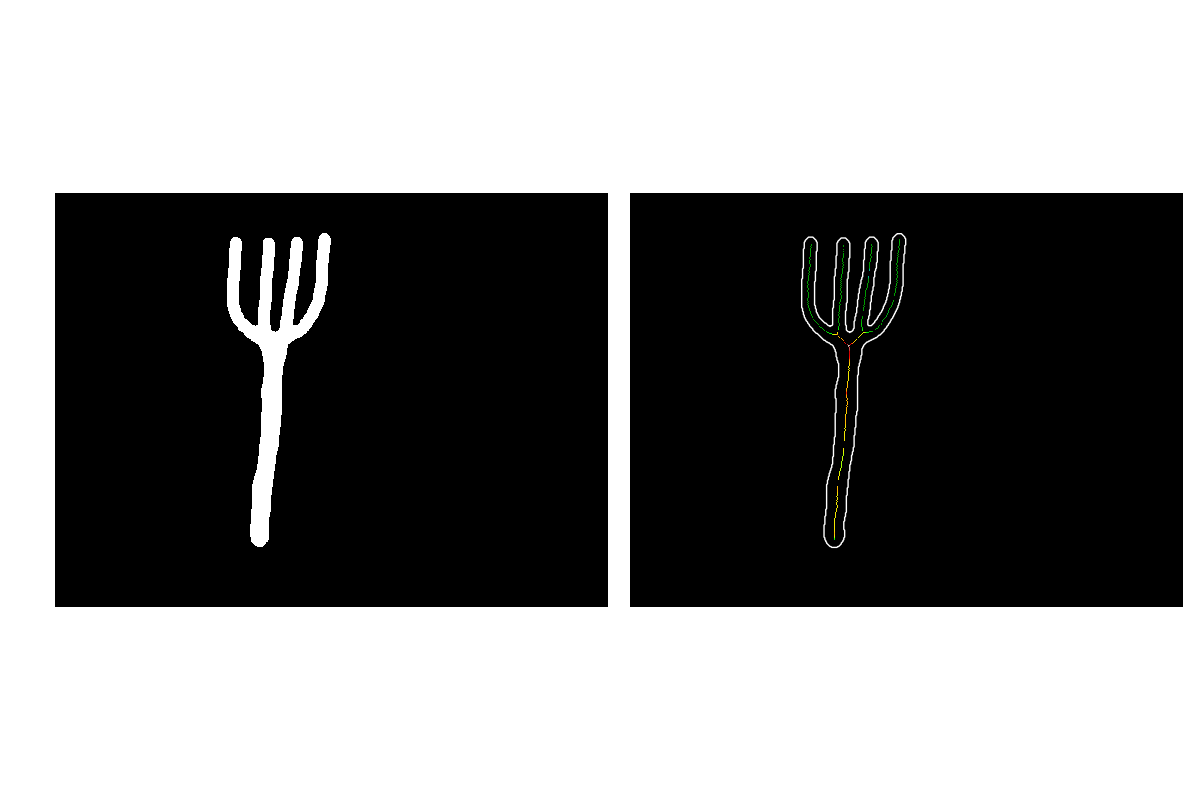
\includegraphics[scale=0.25]{fork_75.png}
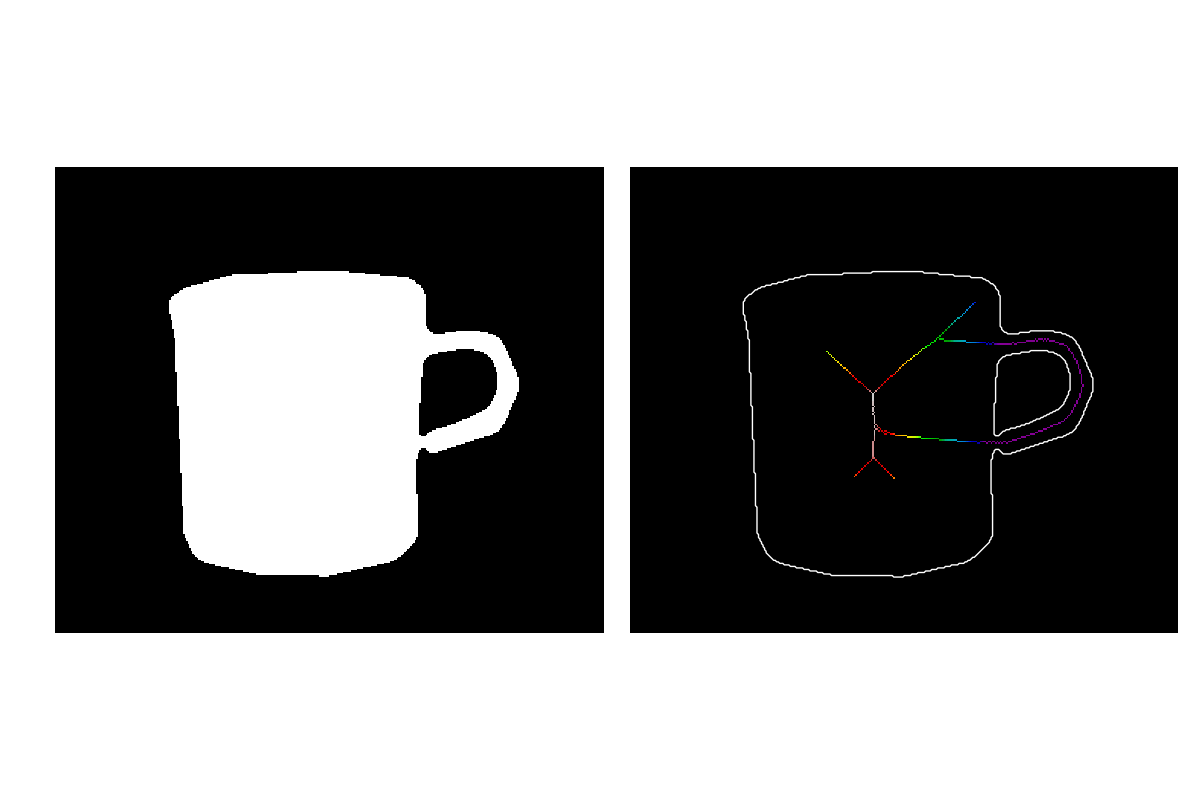
\includegraphics[scale=0.25]{cup_476.png}

\vspace{12px}

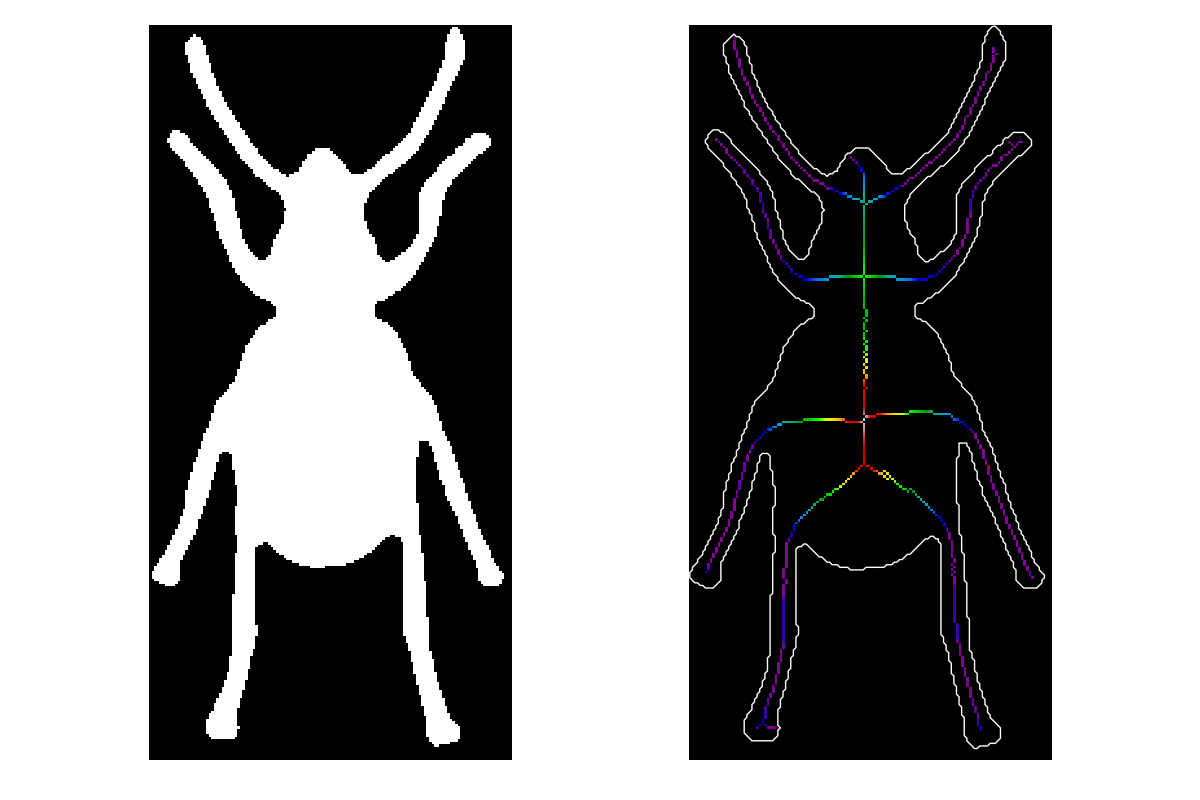
\includegraphics[scale=0.25]{beetle_281.png}
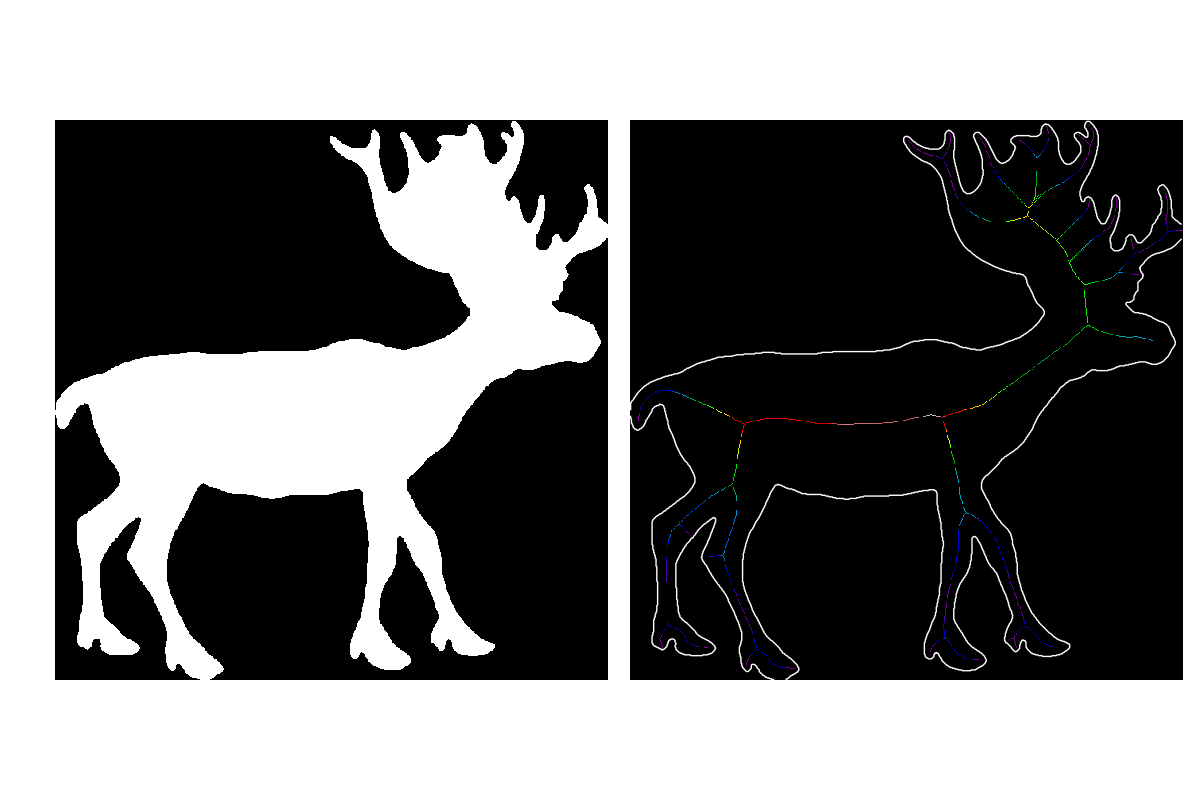
\includegraphics[scale=0.25]{deer_79.png}

\subsubsection{Histogram of distance of the medial axis points from borders}
\subsubsection{Medial axis straight lines}
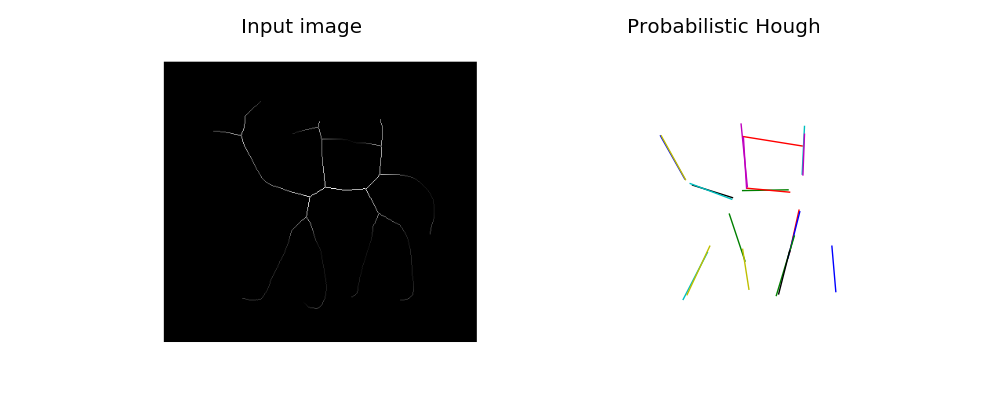
\includegraphics[scale=0.6]{camel_764.png}
\vspace{12px}

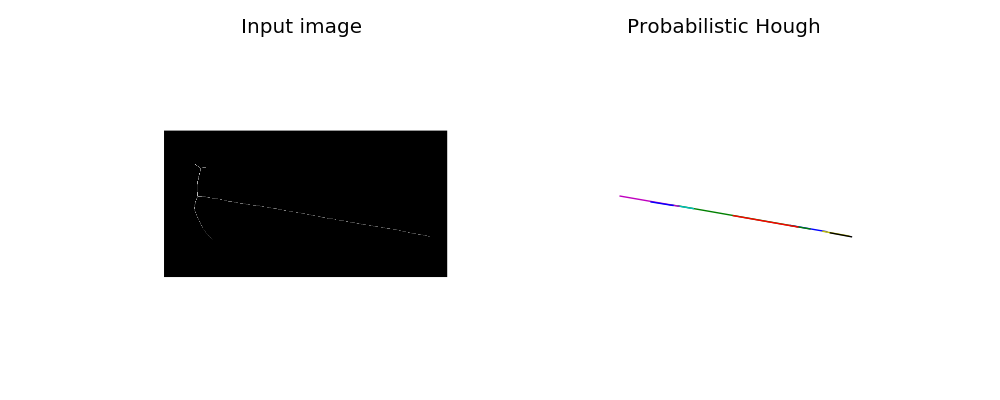
\includegraphics[scale=0.6]{hammer_604.png}

\subsubsection{Quantitive features of skeleton}
To the quantive features of the skeleton the number of branches (number of end points in skeleton)

\subsection{Border Curvature}
\subsubsection{Histogram of border curvature coefficients}

\subsection{Volumetric Features}
\subsubsection{Scaled area}
\subsubsection{Solidity and extend}
\subsubsection{Scaled major and minor axes length}
\subsubsection{Scaled centroid displacement}

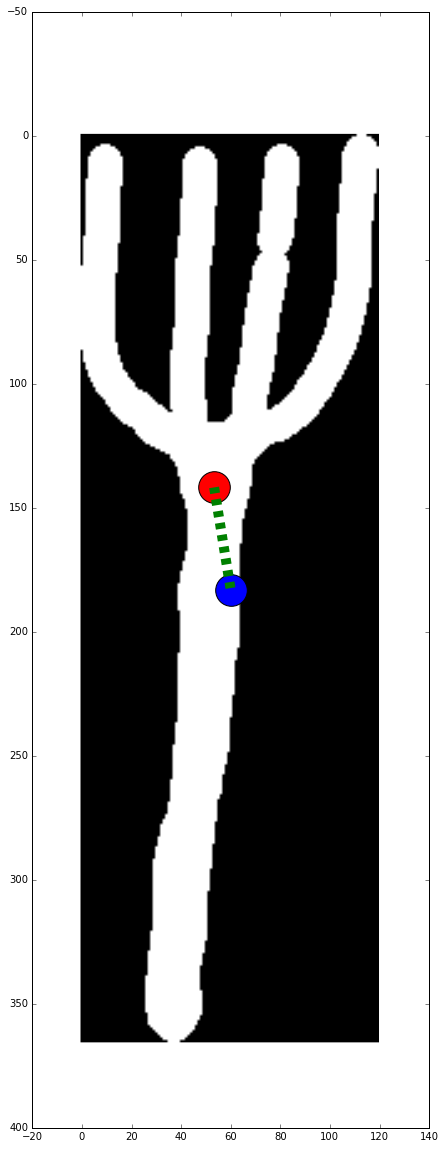
\includegraphics[scale=0.26]{fork_centroid.png}
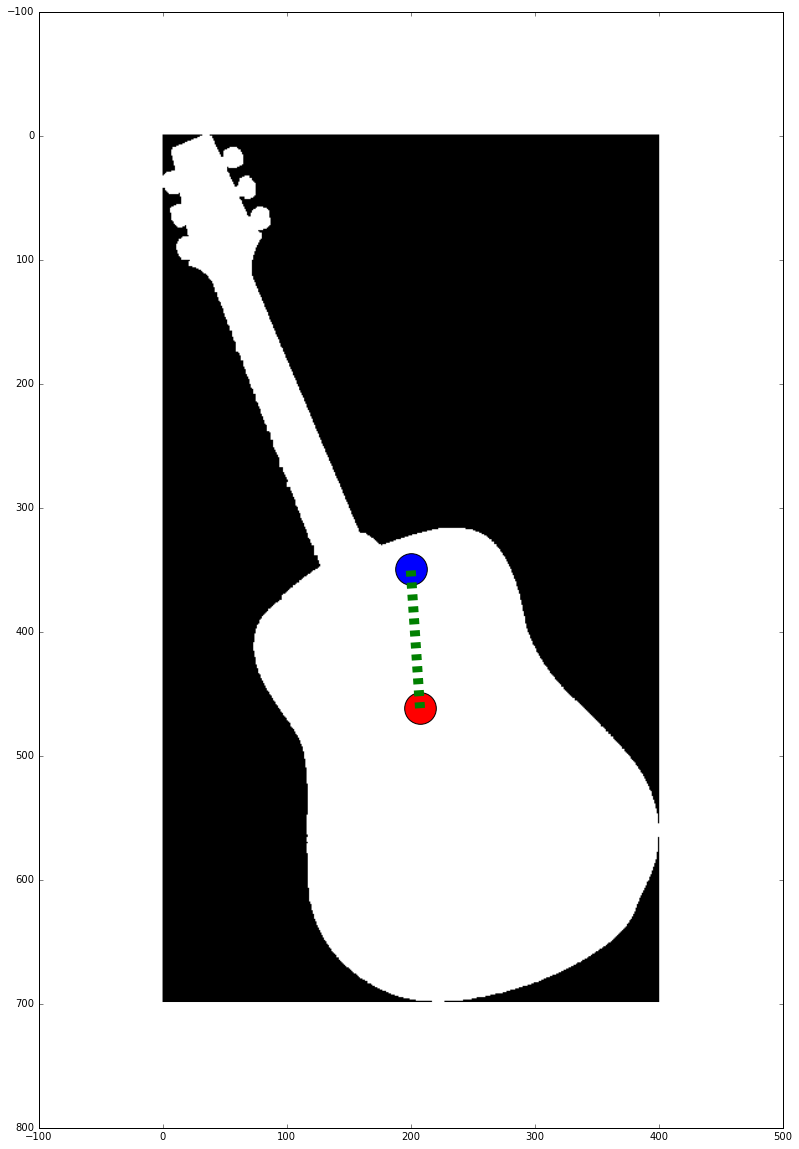
\includegraphics[scale=0.26]{guitar_centroid.png}
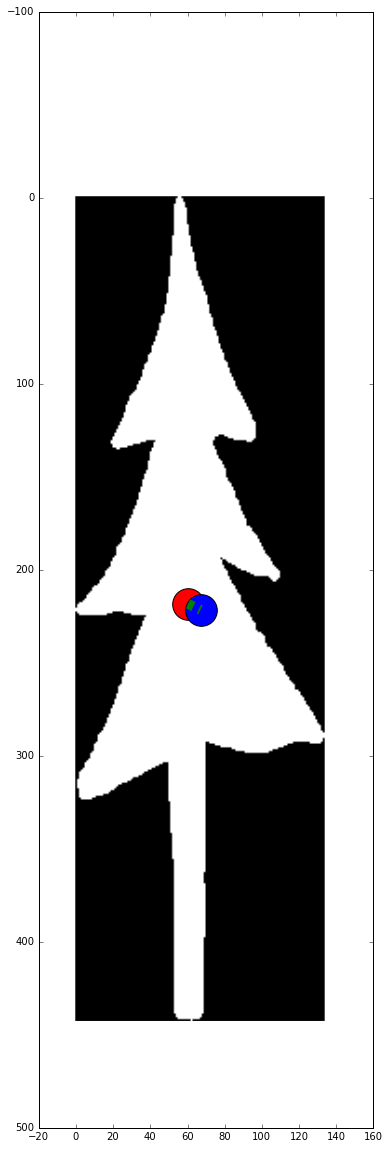
\includegraphics[scale=0.26]{tree_centroid.png}

\subsection{Assymetry measures}
Distances from original image to its horizontal and vertical flips, to rotations for $k*\frac{\pi}/4$
 
\section{Classification models}

Machine Learning techniques were used to build the model of shape recognition. 

Parameters for SVM classifiers were chosen using the grid search according to the best score.

Two kinds of test were performed on the training dataset:
\begin{itemize}
	\item \textbf{Score out of one} class which represents the accuracy score (number of samples with correctly assigned classes over all given samples).
	\item \textbf{Score out of ten} most probable classes which represents the number of samples for which the correct class was found in 10 most probable classes over all given samples.
\end{itemize}

\begin{center}
  \begin{tabular}{| l | c | c |}
    \hline
    \textbf{Classifier} & \textbf{Score out of one} & \textbf{Score out of ten}\\ \hline \hline
    \textit{Gaussian Naive Bayes} & \textit{0.79} & \textit{0.91} \\ \hline
	K-Nearest Neighbours (5 neighbours) & 0.63 & 0.87\\ \hline
	K-Nearest Neighbours (20 neighbours) & 0.5 & 0.92 \\ \hline
	SVM Classifier (linear kernel, C=1) & 0.68 & 0.90 \\ \hline
	\textit{SVM Classifier (RBF kernel, C=10, gamma=0.1)} & \textit{0.78} & \textit{0.93} \\ 
	\hline
  \end{tabular}
\end{center}


\section{Results and Discussions}
\subsection{Performance}
\subsection{Robustness and scale/rotation invariance}
\subsection{Conclusions}

\end{document}
